\documentclass[aspectratio=169,14pt]{beamer}
\usepackage[T1]{fontenc}
\usepackage{lmodern,amsmath,amssymb,booktabs,tabularx,graphicx}
\usepackage{tikz}
\usetikzlibrary{arrows.meta,positioning}
\usefonttheme{professionalfonts}
\definecolor{navy}{HTML}{243746}
\definecolor{blue}{HTML}{2868AE}
\definecolor{muted}{HTML}{626A71}
\definecolor{rust}{HTML}{B04B2C}
\definecolor{teal}{HTML}{1A7D78}
\setbeamercolor{normal text}{fg=navy,bg=white}
\setbeamercolor{structure}{fg=blue}
\setbeamercolor{frametitle}{fg=navy,bg=white}
\setbeamercolor{alerted text}{fg=rust}
\setbeamerfont{frametitle}{size=\Large,series=\mdseries}
\setbeamertemplate{navigation symbols}{}
\setbeamertemplate{itemize items}[circle]
\setbeamersize{text margin left=9mm,text margin right=9mm}
\setlength{\parskip}{4pt}
\setbeamertemplate{footline}{\hfill{\color{muted}\fontsize{8}{9}\selectfont\insertframenumber}\hspace{9mm}\vspace{3mm}}
\newcommand{\source}[1]{\vfill{\fontsize{7.5}{9}\selectfont\color{muted}#1\par}}
\newcommand{\takeaway}[1]{\par\medskip{\color{blue}#1\par}}
\newcommand{\DA}{\operatorname{DA}}
\newcommand{\CH}{\operatorname{H}}
\hypersetup{colorlinks=true,urlcolor=blue,pdfauthor={Ishan Khillan, Elaine Zhang, Todd Zhou}}

\newcommand{\unchangedMenuGain}{14.4}
\newcommand{\unchangedBefore}{13.1}
\newcommand{\unchangedAfter}{27.5}
\newcommand{\subgroupBeforeCount}{304}
\newcommand{\subgroupAfterCount}{638}
\newcommand{\subgroupEntrants}{349}
\newcommand{\subgroupExits}{15}
\newcommand{\ordinaryFixedGainLow}{20.9}
\newcommand{\ordinaryFixedGainHigh}{24.5}
\newcommand{\subgroupGainDev}{14.7}
\newcommand{\subgroupGainPrimary}{14.4}
\newcommand{\subgroupGainRep}{14.9}
\newcommand{\enrichedFixedGainLow}{14.4}
\newcommand{\enrichedFixedGainHigh}{14.9}
\newcommand{\fixedMenuPanelRows}{Ordinary & Jun--Aug 2026 & 1,489 & 19.6 & 40.5 & $+20.9$ [19.1, 22.7]\\
Ordinary & Sep--Oct 2026 & 949 & 23.0 & 44.5 & $+21.6$ [19.7, 23.6]\\
Ordinary & Jun--Aug 2025 & 1,425 & 19.5 & 44.0 & $+24.5$ [22.1, 26.7]\\
Enriched & Jun--Aug 2026 & 2,931 & 11.4 & 26.2 & $+14.7$ [13.9, 15.6]\\
Enriched & Sep--Oct 2026 & 2,328 & 13.1 & 27.5 & $+14.4$ [13.3, 15.5]\\
Enriched & Jun--Aug 2025 & 3,078 & 14.2 & 29.1 & $+14.9$ [13.8, 16.0]\\}
\newcommand{\anchorExits}{37}
\newcommand{\anchorEntrants}{449}
\newcommand{\anchorNet}{412}
\newcommand{\balancedExits}{171}
\newcommand{\balancedEntrants}{1466}
\newcommand{\balancedNet}{1295}

\newcommand{\exactGain}{314}
\newcommand{\retentionGain}{642}
\newcommand{\retentionUpper}{4,620}
\newcommand{\structuralGain}{28}
\newcommand{\structuralCourseExits}{0}
\newcommand{\structuralFamilyExits}{0}
\newcommand{\learnedGain}{50}
\newcommand{\learnedCourseExits}{1}
\newcommand{\learnedFamilyExits}{1}

\hypersetup{pdftitle={Who gets a place? Recommendations under competition}}
\begin{document}

% 1
\begin{frame}[plain]
\vspace{5mm}
{\fontsize{29}{33}\selectfont Who gets a place?\par}
\vspace{5mm}
{\large Recommendations when people compete\\for limited capacity\par}
\vspace{9mm}
Ishan Khillan, Elaine Zhang, Todd Zhou\par
{\small Harvard COMPSCI 2880 / AI for Social Impact\par}
\vfill
{\small November 2026\par}
{\fontsize{7.5}{9}\selectfont\color{muted}The accompanying video uses a synthetic narrator.}
\end{frame}

% 2
\begin{frame}{A better suggestion can hurt someone else}
{\small Two applicants, two seats. A prefers $x$ to $y$. School $x$ gives A priority.}
\medskip
\begin{columns}[T,onlytextwidth]
\begin{column}{.47\textwidth}
\textbf{Before: both get a place}
\begin{center}
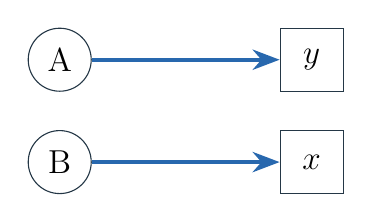
\begin{tikzpicture}[x=1cm,y=1cm,>=Stealth,
 every node/.style={font=\large}, person/.style={circle,draw=navy,minimum size=8mm},
 school/.style={rectangle,draw=navy,minimum size=8mm}]
\node[person] (a) at (0,1.3) {A};
\node[person] (b) at (0,0) {B};
\node[school] (y) at (3.2,1.3) {$y$};
\node[school] (x) at (3.2,0) {$x$};
\draw[->,blue,line width=1.5pt] (a)--(y);
\draw[->,blue,line width=1.5pt] (b)--(x);
\end{tikzpicture}
\end{center}
\end{column}
\begin{column}{.49\textwidth}
\textbf{Change only A's suggestion}
\begin{center}
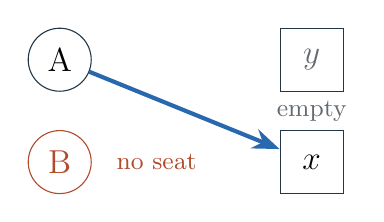
\begin{tikzpicture}[x=1cm,y=1cm,>=Stealth,
 every node/.style={font=\large}, person/.style={circle,draw=navy,minimum size=8mm},
 school/.style={rectangle,draw=navy,minimum size=8mm}]
\node[person] (a) at (0,1.3) {A};
\node[person,draw=rust,text=rust] (b) at (0,0) {B};
\node[school] (x) at (3.2,0) {$x$};
\node[school,text=muted] (y) at (3.2,1.3) {$y$};
\draw[->,blue,line width=1.5pt] (a)--(x);
\node[font=\small,text=rust,anchor=west] at (.6,0) {no seat};
\node[font=\small,text=muted] at (3.2,.65) {empty};
\end{tikzpicture}
\end{center}
\end{column}
\end{columns}
\takeaway{B still sees only $x$. A's new suggestion changes B's outcome.}
\source{Illustrative deferred-acceptance example. Each applicant sees one option. Solid lines show assignments. A's shortlist changes from $\{y\}$ to $\{x\}$; B's shortlist stays $\{x\}$.}
\end{frame}

% 3
\begin{frame}{Choose a shortlist, then assign the places}
A recommender selects a short list of feasible options for each person.
An assignment rule then allocates the available places.

\medskip
\textbf{Matched}\quad Does the person receive any place?\par
\textbf{Target coverage}\quad Is a reference choice on the shortlist?\par
\textbf{Lost match}\quad Was the person matched before, but not after?

\takeaway{Can better recommendations keep everyone who had a place matched somewhere?}
\source{Rental reference: the apartment assigned when all feasible options are shown. Chilean reference: the school in later enrollment. A lost match compares two simulated or replayed allocations, not an observed eviction or revoked offer.}
\end{frame}

% 4
\begin{frame}{Same personal shortlists. Twice the match rate.}
\textbf{Rental simulation: renters with 1--5 feasible apartments.}
These renters saw every feasible option under both policies.
\par\smallskip
Share who receive an apartment:

\bigskip
\begin{columns}[T,onlytextwidth]
\begin{column}{.45\textwidth}\centering
{\fontsize{32}{36}\selectfont\unchangedBefore\%\par}
Anchor: coordinate one option
\end{column}
\begin{column}{.45\textwidth}\centering
{\fontsize{32}{36}\selectfont\color{blue}\unchangedAfter\%\par}
Balance the whole shortlist
\end{column}
\end{columns}
\bigskip
\textbf{Only other renters' shortlists changed.}
\source{Sep--Oct 2026 enriched simulation, 2,328 renter appearances. Anchor + GPT versus Balanced + GPT. Match rates are seed means. The gain is 14.41 percentage points; 15 previously matched members of this group become unmatched. Repeated appearances are not unique households.}
\end{frame}

% 5
\begin{frame}{Why study rentals and school admissions?}
\small
\renewcommand{\arraystretch}{1.35}
\begin{tabularx}{\textwidth}{@{}p{2.1cm}XX@{}}
\toprule
Setting & What it lets us examine & Evidence boundary\\\midrule
NYC rentals & Actual cached GPT shortlists and alternative coordination rules & Market inputs, modeled preferences and allocations\\
Chile schools & Submitted rankings, actual admission rules and recipient protection & Observed reports and outcomes, counterfactual new shortlists\\
\bottomrule
\end{tabularx}
\par\medskip
\normalsize
The common mechanism is competition for limited capacity.\par
The settings answer different parts of the question.
\source{Rentals: 1,280 markets, three reused calendar windows, two designs; 320 original supply failures. Chile: about 2.04 million audited applicant-years in 2022--25, about 1.97 million linked to enrollment. Jobs provide a secondary coordinated-baseline check in the appendix.}
\end{frame}

% 6
\begin{frame}{Two ways to coordinate recommendations}
\textbf{One anchor}\par
Find a maximum feasible matching. Put each assigned option on its recipient's shortlist.

\medskip
\textbf{Balanced shortlists}\par
Minimize squared listing exposure with exact min-cost flow.
Use saved GPT ranks to choose among equally balanced shortlists.

\medskip
Shortlist lengths stay fixed. The anchor replaces at most one option per person; balancing can replace several.
\source{Both use feasibility and saved recommendations. They do not see realized preference shocks, landlord priorities or reference assignments. The anchor maximizes reuse among maximum matchings.}
\end{frame}

% 7
\begin{frame}{Individual coverage misses the placement loss}
\begin{center}
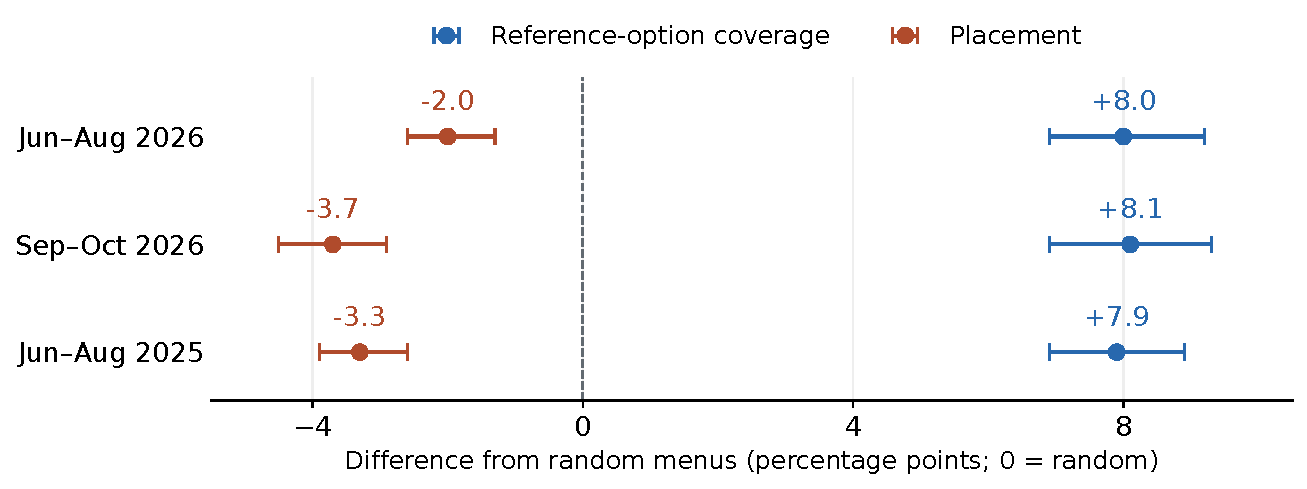
\includegraphics[width=.94\textwidth]{figures/rentals.pdf}
\end{center}
\takeaway{Higher reference coverage does not imply more placements.}
\source{Enriched markets select cheaper listings and renters with feasible options. GPT minus random, 95\% market-bootstrap intervals. Coverage conditions on a full-list match. Properties recur across windows.}
\end{frame}

% 8
\begin{frame}{Coordination changes the comparison}
\begin{center}
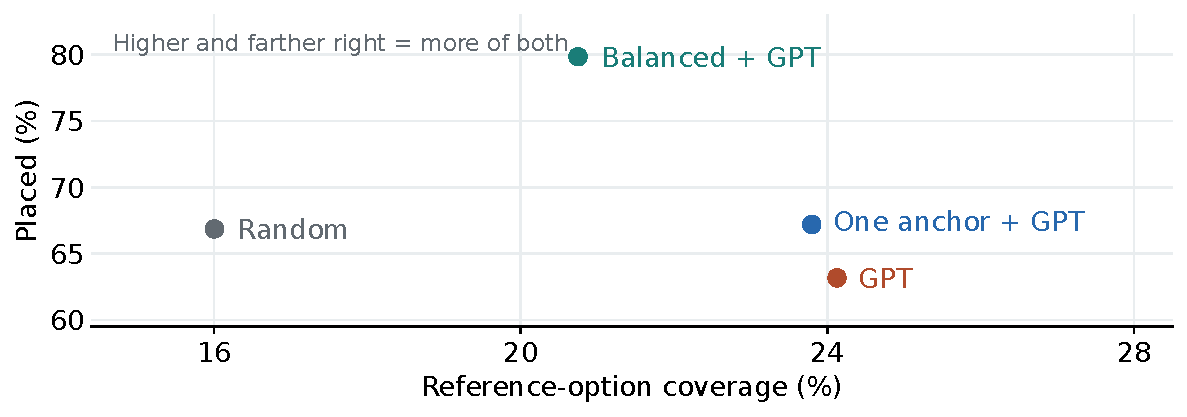
\includegraphics[width=.92\textwidth]{figures/rental-policies.pdf}
\end{center}
\takeaway{Balanced shortlists improve both outcomes over random shortlists.}
\source{Sep--Oct 2026 enriched replay, point means. Placement: random 66.9\%, GPT 63.2\%, anchor 67.2\%, balanced 79.8\%. The comparison with the anchor loses 3.05 coverage points and gains 12.65 placement points. A control with simulator-utility information improves both metrics further. All panels and paired intervals are in the appendix.}
\end{frame}

% 9
\begin{frame}{A net gain does not tell us who gained}
{Anchor versus original GPT, on the same rental markets.}
\bigskip
\begin{columns}[T,onlytextwidth]
\begin{column}{.30\textwidth}\centering
{\fontsize{31}{35}\selectfont\color{blue}\anchorEntrants\par}
newly placed
\end{column}
\begin{column}{.30\textwidth}\centering
{\fontsize{31}{35}\selectfont\color{rust}\anchorExits\par}
previously placed,\\now unplaced
\end{column}
\begin{column}{.30\textwidth}\centering
{\fontsize{31}{35}\selectfont\anchorNet\par}
net gain
\end{column}
\end{columns}
\bigskip
The stronger balancing policy also displaces prior recipients:
\alert{\balancedExits{} exits} relative to the anchor.
\source{Sep--Oct 2026 enriched replay, 10,240 renter appearances. $449-37=412$. GPT places 6,469 appearances; the anchor places 6,881. Balancing has 1,466 entrants and 171 exits relative to the anchor. Counts are not unique households or observed evictions.}
\end{frame}

% 10
\begin{frame}{Why can an unchanged shortlist help you?}
Renters with \textbf{one to five feasible listings} already see every option.

\medskip
\begin{center}
\small
\renewcommand{\arraystretch}{1.45}
\begin{tabular}{l@{\hspace{12mm}}r}
\toprule
Policy applied to the whole market & This group's match rate\\\midrule
One anchor + GPT & \unchangedBefore\%\\
Balanced + GPT & \unchangedAfter\%\\
\bottomrule
\end{tabular}
\end{center}
\takeaway{The \unchangedMenuGain-point gain comes from changes to other people's shortlists.}
\source{Sep--Oct 2026 enriched replay, 2,328 subgroup appearances. Mean within-seed match rates; paired difference 14.41 pp, pointwise 95\% interval [13.27,15.51]. The subgroup still has 15 exits under balancing. This is a simulated spillover, not a field effect.}
\end{frame}

% 11
\begin{frame}{Chile: the losses are concentrated}
{More enrollment hits under rank-informed shortlists, fewer placements.}
\begin{center}
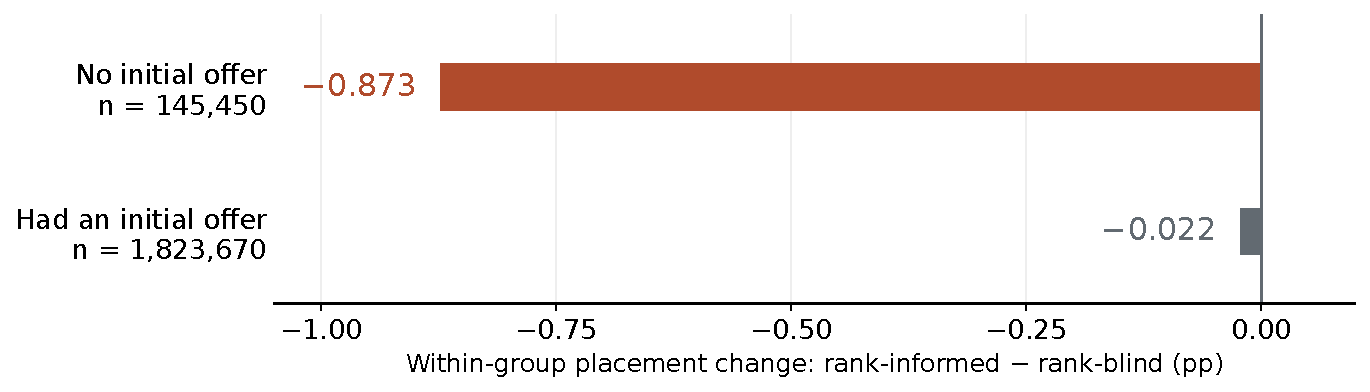
\includegraphics[width=.86\textwidth]{figures/chile-incidence.pdf}
\end{center}
\textbf{No historical offer: 7.4\% of the sample, 76.0\% of the net loss.}
\source{Rank-informed versus rank-blind classifiers, trained to predict initial offers. Coverage instead targets later enrollment. 2022--25 linked applicant-years; fixed reported preferences. No-offer group loses 1,270 of 1,670 net placements. These are counterfactual losses, not revoked official offers.}
\end{frame}

% 12
\begin{frame}{The comparison policy matters}
Same rank-informed shortlists. Same linked Chilean cohorts.

\medskip
\small
\renewcommand{\arraystretch}{1.35}
\begin{tabularx}{\textwidth}{@{}Xr@{\hspace{5mm}}r@{}}
\toprule
Compared with & Enrollment hits & Placements\\\midrule
Rank-blind shortlists & $+4,638$ & $-1,670$\\
First five discretionary courses & $+9,800$ & $+8,143$\\
\bottomrule
\end{tabularx}
\par\medskip
\normalsize
Even against first-five, pupils without a historical offer lose \alert{2,860 placements}.
\takeaway{Better aggregate outcomes do not settle the access question.}
\source{Counterfactual allocations with fixed reports. Historical-school coverage is not a welfare measure. Sources: findings/chile/cohort\_comparison.csv and group\_comparison.csv.}
\end{frame}

% 13
\begin{frame}{Choosing shortlists with zero exits is hard}
Choose one shortlist policy $D$ for a supplied set of priority draws $S$:
\[
\max_{D\in\mathcal D}\ H(D)-H(A)
\qquad\text{subject to}\qquad X_s(D;A)=0\quad\forall s\in S.
\]
\small
$A$: baseline (rank-blind in Chile). \quad $H$: number of reference hits.\par
$X_s$: baseline recipients left unplaced on draw $s$.\par
$\mathcal D$: keep shared options, fill from both policies' union, keep quotas.

\medskip
\normalsize
\textbf{Theorem.} Reaching a target gain is NP-complete, even with unit seats and shortlists of length at most three.
\source{Fixed strict responsive priorities, with one common priority order per supplied draw in the reduction. DA checks a proposed policy in polynomial time. Independent Set reduction and stable-witness formulation are in the appendix. Chile's family rules are evaluated separately.}
\end{frame}

% 14
\begin{frame}{Why individually safe edits can conflict}
{\small One priority draw for edge $\{u,v\}$; $h_u,h_v$ already have seats.}
\begin{center}
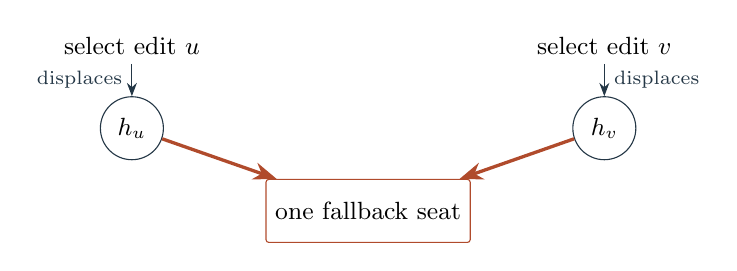
\begin{tikzpicture}[x=1cm,y=1cm,>=Stealth,
 every node/.style={font=\small}, pupil/.style={circle,draw=navy,minimum size=8mm},
 seat/.style={rectangle,draw=rust,rounded corners=1pt,minimum width=24mm,minimum height=8mm}]
\node (u) at (0,1) {select edit $u$};
\node (v) at (6,1) {select edit $v$};
\node[pupil] (hu) at (0,-.05) {$h_u$};
\node[pupil] (hv) at (6,-.05) {$h_v$};
\node[seat] (z) at (3,-1.1) {one fallback seat};
\draw[->,navy] (u)-- node[left,font=\scriptsize]{displaces} (hu);
\draw[->,navy] (v)-- node[right,font=\scriptsize]{displaces} (hv);
\draw[->,rust,line width=1.2pt] (hu)--(z);
\draw[->,rust,line width=1.2pt] (hv)--(z);
\end{tikzpicture}
\end{center}
Either edit alone is safe; together, one pupil loses a seat.

\medskip
The same edit set must work on \textbf{every} draw.\par
No selected pair can share an edge: an independent set.
\source{Proof intuition. Other vertex edits are harmless on this edge's draw. Each selected vertex adds one reference hit. The appendix gives the full preferences, private schools, reference draw and polynomial-size construction.}
\end{frame}

% 15
\begin{frame}{Allowing school switches leaves more room}
{\small Same allowed shortlists, same 1,024 design lotteries per cohort.}
\medskip
\small
\renewcommand{\arraystretch}{1.5}
\begin{tabularx}{\textwidth}{@{}Xr@{\hspace{5mm}}r@{}}
\toprule
Protection & Achieved gain & Upper bound\\\midrule
Same course and seat type & $\exactGain$ & $\exactGain$\\
A seat retained, school may change & $\retentionGain$ & $\retentionUpper$\\
\bottomrule
\end{tabularx}
\par\medskip
\normalsize
Switches permit more than twice the demonstrated coverage gain.

\medskip
We have not solved the retention problem to optimality.
\source{Additional enrollment hits, summed over the 2022--24 cohort problems. A hindsight optimization bracket, not a confidence interval or a deployable effect estimate. Retaining a seat does not guarantee a preferred school. Source: findings/chile/retention\_bounds.csv.}
\end{frame}

% 16
\begin{frame}{A test panel is weaker than a guarantee}
Choose rules before assignment, using submitted applications.
\par\medskip
\small
\renewcommand{\arraystretch}{1.3}
\begin{tabularx}{\textwidth}{@{}Xr@{\hspace{5mm}}r@{\hspace{4mm}}r@{}}
\toprule
Rule & Hit gain & \multicolumn{2}{c}{Incumbent exits}\\
 & & Course & Family\\\midrule
Structural rule, all-order proof & $+\structuralGain$ & $\structuralCourseExits$ & $\structuralFamilyExits$\\
Learned rule, design-panel checks & $+\learnedGain$ & $\learnedCourseExits$ & $\learnedFamilyExits$\\
\bottomrule
\end{tabularx}
\par\medskip
\normalsize
The proven rule gives a small gain.\par
The learned rule fails the zero-exit promise on fresh draws.
\source{2022--24: 384 course cohort-draws and 96 school/family cohort-draws. Gains count historical hits once, not per draw. The proof assumes fixed inputs and the reconstructed mechanism. Neither rule improves coverage for the historical no-offer group.}
\end{frame}

% 17
\begin{frame}{Protecting recipients can preserve exclusion}
The structural Chile rule protects incumbents, but adds \textbf{no new entrants} in the paired test lotteries.

\medskip
An access objective must also count people who start without a place.
Historical enrollment and modeled ranks are incomplete welfare measures.

\medskip
Before deployment: preserve the ability to add choices, audit displaced people, and provide human review or appeal.
\source{Zero entrants is a result for the reported structural-rule panels, not a general impossibility. The safeguards are proposed, not evaluated. A recommendation redistributes existing opportunities; it does not create affordable housing or school capacity.}
\end{frame}

% 18
\begin{frame}{Evaluate the allocation, not just the list}
Better coordination can improve coverage and placement together.

\medskip
Individual retention is a separate requirement, with its own computational difficulty.

\bigskip
{\large The next design problem:\par
Improve access for people without a place\\while protecting those who already have one.}
\vfill
{\color{muted}Thank you.}
\end{frame}
\end{document}
